%% ============================================================
%% Revision Notes (2026-03-29, Yuyang):
%% 1. Core Principle: Removed mathematical formulation (autoregressive
%%    equation) and decoding strategy enumeration. Kept concise prose
%%    description of real-time logit/probability manipulation.
%% 2. Applications: Merged sub-categories (Contrastive/External Guidance/
%%    Context-Adaptive/Specialized/Reference-Based etc.) into one
%%    paragraph per trustworthiness domain. Removed \textbf sub-headings.
%% 3. Discussion: Removed from this file. Shortened version moved to
%%    sections/11-challenges_directions.tex with red source marker.
%% ============================================================

\subsection{Decoding}
\label{sec:decoding}

\begin{figure}[htbp]
\centering
% Width uses \textwidth; height auto-scales with !
\resizebox{\textwidth}{!}{%
\begin{tikzpicture}
% --- 1. Define leaf nodes (papers, citations added) ---
\node[leaf] (safety_papers) {
Adversarial Contrastive Decoding~\citep{Zhao2024AdversarialCD}, Alignment-Enhanced Decoding~\citep{Liu2024AlignmentEnhancedDD}, ROSE~\citep{Zhong2024ROSEDD}, SafeDecoding~\citep{Xu2024SafeDecodingDA}, SafeAligner~\citep{Huang2024SafeAlignerSA}, Zeng et al.~\citep{Zeng2024RootDS}, MoGU~\citep{Du2024MoGUAF}, Controllable Safety Alignment~\citep{Zhang2024ControllableSA}, MetaSC~\citep{Gallego2025MetaSCTS}, FlexLLM~\citep{Chen2024FlexLLMEL}, SafeInfer~\citep{Banerjee2024SafeInferCA}, CoCA~\citep{Gao2024CoCARS}, Immune~\citep{Ghosal2024ImmuneIS}, CleanGen~\citep{Li2024CleanGenMB}.
};
\node[leaf, below=0.3cm of safety_papers] (factuality_papers) {
Octopus~\citep{Suo2025OctopusAH}, HELPD~\citep{Yuan2024HELPDMH}, ConVis~\citep{Park2024ConVisCD}, Liang et al.~\citep{Liang2024MitigatingHI}, Chen et al.~\citep{Chen2024LowerLM}, Huang et al.~\citep{Huang2025DynamicAC}, DeCo~\citep{Wang2024MLLMCS}, Bi et al.~\citep{Bi2024DecodingBC}, Reference Trustable Decoding~\citep{Shi2024ReferenceTD}.
};
\node[leaf, below=0.3cm of factuality_papers] (fairness_papers) {
Dhamala et al.~\citep{Dhamala2022AnAO}, Das et al.~\citep{Das2022QuantifyingBF}.
};
\node[leaf, below=0.3cm of fairness_papers] (privacy_papers) {
Privacy-Aware Decoding~\citep{Wang2025PrivacyAwareDM}, Ok et al.~\citep{Ok2024DecodingWL}, Wei et al.~\citep{Wei2024PrivacyRO}, Borec et al.~\citep{Borec2024TheUI}, Majmudar et al.~\citep{Majmudar2022DifferentiallyPD}, Isonuma et al.~\citep{Isonuma2024WhatsNI}.
};
% --- 2. Define main sub-nodes (Trustworthiness dimensions) ---
% Positioned to the left of corresponding leaf nodes
\node[sub, left=0.5cm of safety_papers] (safety) {Safety};
\node[sub, left=0.5cm of factuality_papers] (factuality) {Factuality \& Faithfulness};
\node[sub, left=0.5cm of fairness_papers] (fairness) {Fairness};
\node[sub, left=0.5cm of privacy_papers] (privacy) {Privacy};
% --- 3. Define root node ---
% Use the calc library to vertically center the root node relative to the sub-nodes
\node[main, left=2.5cm of {$(safety.west)!0.5!(privacy.west)$}] (decoding) {Decoding (§\ref{sec:decoding})};
% --- 4. Draw connection lines ---
% a. Draw a main trunk from the root node to a branching point
\coordinate (fork) at ($(decoding.east)+(1.25cm,0)$);
\draw[line] (decoding.east) -- (fork);
% b. Connect from main branching point to each sub-node
\draw[line] (fork) |- (safety.west);
\draw[line] (fork) |- (factuality.west);
\draw[line] (fork) |- (fairness.west);
\draw[line] (fork) |- (privacy.west);
% c. Connect main sub-nodes directly to leaf nodes
\draw[line] (safety.east) -- (safety_papers.west);
\draw[line] (factuality.east) -- (factuality_papers.west);
\draw[line] (fairness.east) -- (fairness_papers.west);
\draw[line] (privacy.east) -- (privacy_papers.west);
\end{tikzpicture}%
}
\caption{A taxonomy of Decoding Strategies for enhancing LLM trustworthiness.}
\label{fig:decoding_taxonomy}
\end{figure}

\subsubsection{Core Principle: Real-Time Logit and Probability Manipulation}

Decoding strategies involve real-time manipulation of the token probability distribution or logits at each generation step to steer the model's outputs toward desired characteristics. At each step, the model produces a probability distribution over its vocabulary conditioned on the preceding tokens, and decoding interventions modify this distribution---by suppressing, amplifying, or re-weighting specific token probabilities---before sampling the next token. This approach allows for fine-grained control over output without modifying the model's parameters, making it computationally efficient and adaptable to diverse trustworthiness requirements.

\begin{figure*}[htbp]
  \centering
  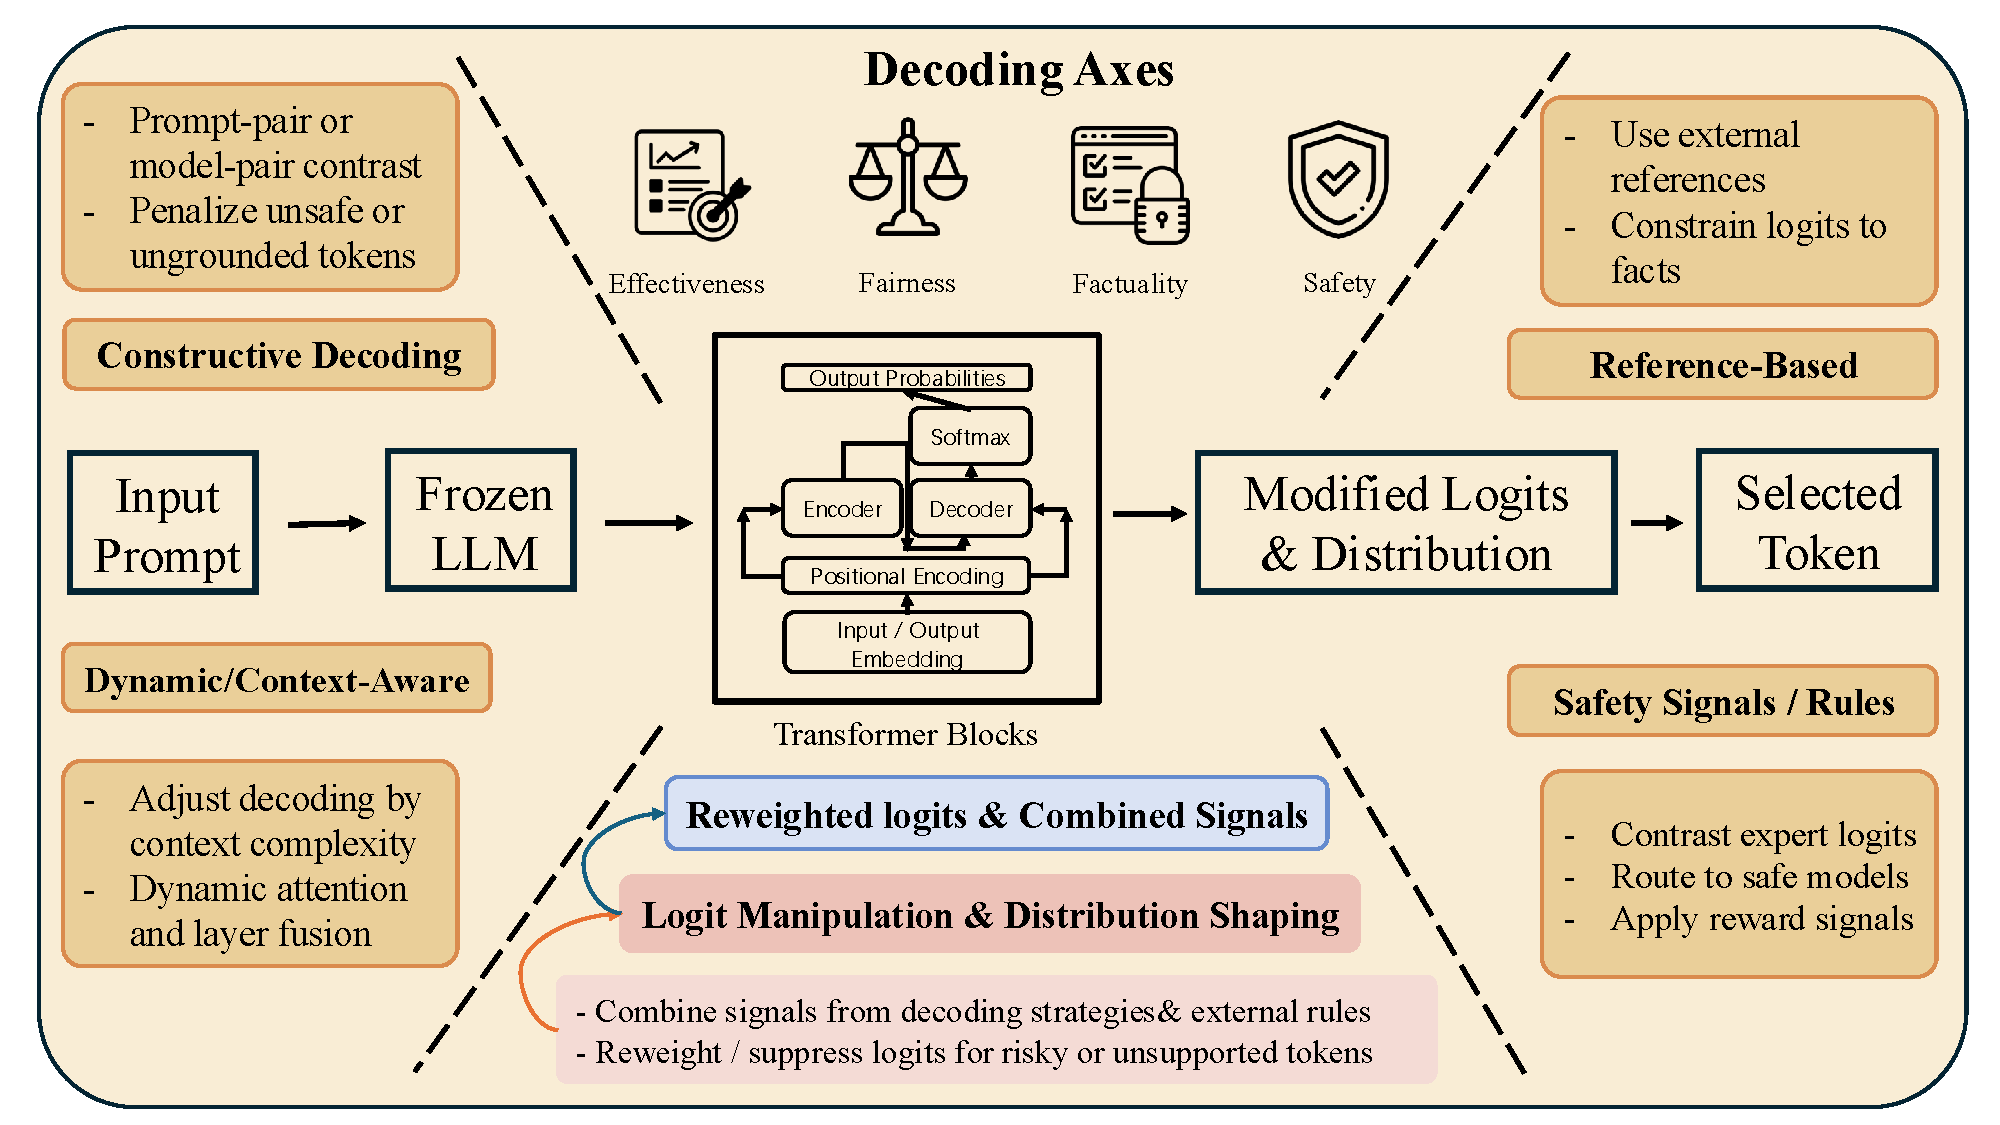
\includegraphics[width=0.9\linewidth]{figures/method/decoding_new2.pdf}
  \caption{Overview of trustworthiness-oriented decoding strategies. A frozen LLM produces logits that are modified at each autoregressive step by three complementary families of interventions before token sampling. \textbf{Contrastive Decoding} (balance icon) contrasts outputs from paired prompts or paired models---e.g., safe versus unsafe prompts, or an expert against an amateur model---to penalize unsafe or ungrounded tokens. \textbf{Dynamic/Context-Aware Decoding} (neural-network icon) adjusts decoding hyperparameters, attention weights, or layer fusion on the fly, based on context complexity or intermediate signals. \textbf{Reference-Based Decoding} (document-with-shield icon) constrains logits toward facts or safety policies sourced from external references such as retrieved documents or rule sets. These three families feed into a shared \emph{Logit Manipulation \& Distribution Shaping} stage, optionally combined with external knowledge or safety signals, which reweights or suppresses risky, unsupported, or unsafe tokens before the next token is sampled.}
  \label{fig:method_decoding}
\end{figure*}


\subsubsection{Applications}

\paragraph{Safety}

Decoding strategies for safety center on inference-time intervention to prevent harmful outputs without altering model weights, and are crucial for defending against adversarial attacks such as jailbreaks. Contrastive decoding enhances safety by comparing logits from safe and unsafe distributions: methods like Adversarial Contrastive Decoding~\citep{Zhao2024AdversarialCD} and Alignment-Enhanced Decoding~\citep{Liu2024AlignmentEnhancedDD} use opposite or malicious prompts to penalize unsafe continuations, while SafeDecoding~\citep{Xu2024SafeDecodingDA} and SafeAligner~\citep{Huang2024SafeAlignerSA} contrast logits from safety-trained expert models against base or unsafe models, and ROSE~\citep{Zhong2024ROSEDD} applies reverse prompt contrastive decoding with step-by-step correction~\citep{Zeng2024RootDS}. External guidance approaches use separate models or signals to steer generation, such as MoGU's dynamic routing between a usable and a safe LLM~\citep{Du2024MoGUAF}, inference-time adaptation through safety configurations~\citep{Zhang2024ControllableSA}, and meta-critique optimization of safety specifications~\citep{Gallego2025MetaSCTS}. Context-adaptive and dynamic defenses adjust safety measures based on specific inputs, including moving target defense through dynamic decoding hyper-parameters~\citep{Chen2024FlexLLMEL} and context-adaptive safety amplification~\citep{Banerjee2024SafeInferCA}. Specialized defense work addresses safety in multimodal LLMs through output distribution calibration~\citep{Gao2024CoCARS} and safety reward model alignment~\citep{Ghosal2024ImmuneIS}, as well as countering backdoor attacks via speculative decoding to identify suspicious tokens~\citep{Li2024CleanGenMB}.

\paragraph{Factuality}

Diverse decoding strategies have been developed to mitigate hallucinations and ensure context-aware outputs in LLMs and MLLMs. Contrastive decoding reduces hallucinations by contrasting output distributions derived from original and perturbed inputs: Octopus~\citep{Suo2025OctopusAH} adapts to input complexity with noise, HELPD~\citep{Yuan2024HELPDMH} employs hierarchical feedback with vision-enhanced penalty decoding, ConVis~\citep{Park2024ConVisCD} penalizes hallucinated content via text-to-image reconstruction, and further methods re-balance distributions to prioritize visual grounding~\citep{Liang2024MitigatingHI} or integrate multi-layer fusion with contrastive decoding~\citep{Chen2024LowerLM}. Context-aware decoding dynamically adjusts strategies to ensure faithfulness to input context, such as dynamically adjusting attention mechanisms to prioritize context-relevant tokens~\citep{Huang2025DynamicAC} and adaptively selecting preceding layers to correct output logits~\citep{Wang2024MLLMCS}. Reference-based decoding enhances factual consistency by contrasting knowledge states to improve confidence on edited facts~\citep{Bi2024DecodingBC} or using reference information to ensure output consistency without additional training~\citep{Shi2024ReferenceTD}.

\paragraph{Privacy}

Decoding strategies address privacy concerns by targeting two objectives: reducing privacy leakage and reducing memorization. For leakage prevention, Privacy-Aware Decoding~\citep{Wang2025PrivacyAwareDM} filters outputs in RAG systems to prevent disclosure of sensitive retrieved data, selective teacher supervision during decoding avoids leaking data from untrusted sources~\citep{Ok2024DecodingWL}, and privacy vulnerabilities in speculative decoding have been identified where accelerated inference may increase leakage risks~\citep{Wei2024PrivacyRO}. For memorization reduction, nucleus sampling has been shown to only modestly reduce memorization due to peaked output distributions~\citep{Borec2024TheUI}, differential privacy applied during decoding by adding noise to logits provides formal guarantees~\citep{Majmudar2022DifferentiallyPD}, and contrastive generation encourages novel outputs to reduce reliance on memorized training data~\citep{Isonuma2024WhatsNI}.

\paragraph{Fairness}

While decoding strategies have been explored for safety, factuality, and privacy, their impact on fairness remains a nascent and under-explored domain. Dhamala et al.~\citep{Dhamala2022AnAO} provide a pioneering analysis of how decoding parameters such as top-$k$, top-$p$, and temperature sampling influence fairness in open-ended text generation, demonstrating that specific hyperparameter configurations can exacerbate or mitigate group-level disparities. Similarly, Das et al.~\citep{Das2022QuantifyingBF} explore bias across the entire decoder hyperparameter space, revealing critical trade-offs between bias reduction and generation quality. These studies highlight fairness as an emerging frontier in decoding methods, where systematic methodologies and robust interventions remain a pressing need.
